% Generated from: Zhihu/专栏：概率与统计/渐近统计 (10)：U-统计量 (上)_金鱼马_2026-06-06.md

U-统计量 (U-statistics) 的基本理论最早由 W. Hoeffding 在其 1948 年的经典论文 \emph{A Class of Statistics with Asymptotically Normal Distribution} 中系统性地提出\cite{hoeffding1948}。其中的``U''取无偏 (unbiased) 之意。

U-统计量在非参数估计中有广泛应用：

\begin{itemize}
\item
  不少用于估计经典统计量，在形式上都是 U-统计量，例如样本均值和无偏样本方差，更复杂的例子有 Mann--Whitney 估计和 Kendall's $\tau$。
\item
  利用 U-统计量可以进行诸多推断：如进行方差估计、构造置信区间；在假设检验问题中，基于 U-统计量的置换检验和秩检验有着不依赖总体分布假设的优点。
\item
  即使是现代机器学习中，诸如 AUC（曲线下面积）、基于最大均值差异 (MMD) 核的两样本检验、基于 HSIC 统计量的独立性检验等技术，都可以由 U-统计量得出；这里甚至包括著名的 GRPO\cite{zhou2026grpo}。为了解决计算成本高昂的问题，人们还发展出了``不完全 U-统计量 (incomplete U-statistics)''的技术。
\end{itemize}

这种统计量自提出起就受到概率统计学者们的很大重视，可以参考的介绍性资料包括但不限于：

\begin{itemize}
\item
  Serfling 的 \emph{Approximation Theorems of Mathematical Statistics} 第 5 章\cite[Chapter~5]{serfling1980}；
\item
  Lee 的 \emph{U-Statistics: Theory and Practice}\cite{lee1990}；
\item
  van der Vaart 的 \emph{Asymptotic Statistics} 第 12 章\cite[Chapter~12]{vandervaart1998}；
\item
  Lehmann 的 \emph{Elements of Large-Sample Theory} 第 6 章\cite[Chapter~6]{lehmann1999}；
\item
  陈希孺、方兆本等的《非参数统计》第二章\cite[第 2 章]{chenxiru2012}；
\item
  Lehmann 和 Romano 的 \emph{Testing Statistical Hypotheses} 第 12 章\cite[Chapter~12]{lehmannromano2022}；
\item
  Thomas S. Ferguson 的 U-统计量讲义\cite{fergusonustat}。
\end{itemize}

% 我们今天主要介绍 U-统计量的基本概念、应用、以及初步的渐近性质。

\section{基本概念}

\subsection{统计泛函与插入估计}\label{sec:ch10a:plug-in}

设 $P$是样本空间 $(\mathscr X,\mathscr B_x)$ 上的概率分布，来自某分布族 $\mathscr P$ ；那么一个\textbf{\emph{统计泛函}} (statistical functional) 是 $P$ 的函数 $\theta: P\mapsto \theta(P)\in\mathbb R$ ，例如

\begin{itemize}
\tightlist
\item
  均值 $\mu(P)=\int_{\mathscr X}x\mathrm{d}P(x)=\mathbb{E}_P[X]$ 和方差 $\sigma^2(P)=\int_{\mathscr X}(X-\mu)^2\mathrm{d}P(x)=\mathrm{Var}_P[X]$ ，以及各阶矩；
\item
  偏度 $P\mapsto \mathbb{E}_P\left[\left(\tfrac{X-\mu}{\sigma}\right)^3\right]$ 和峰度 $P\mapsto\mathbb{E}_P\left[\left(\tfrac{X-\mu}{\sigma}\right)^4\right]-3$ ；
\item
  分布函数 $P\mapsto F(t)=P(X\le t)$ ，其中 $t$ 固定；
\item
  中位数 $m(P)=F^{-1}(\tfrac12)=\inf\left\{x\in\mathbb R:P(X\le x)\ge \tfrac12\right\}$ ；
\item
  Gini 平均差 $P\mapsto \int_{\mathscr X}\!\int_{\mathscr X}|x_1-x_2|\mathrm dP(x)\mathrm dP(x_2)=\mathbb E_P[|X_1-X_2|]$ ；
\end{itemize}

设 $X_1,\dots,X_n\sim P$ 是 i.i.d. 样本， $\mathbb P_n:=\frac1n\sum_{j=1}^n\delta_{X_j}$ 是经验分布，那么对统计泛函 $\theta_0=\theta(P)$ ，用 $\widehat\theta=\theta(\mathbb P_n)$估计之，是很自然的选择，这被称作\textbf{\emph{插入估计}} (plug-in estimator)。

进一步，如果 $\theta$ 满足：存在某 $m$ 个样本（ $m\le n$ ）的 Borel 可测函数 $h:\mathscr X^m\to\mathbb R$ ， $\mathbb E_P[|h(X_1,\dots,X_m)|]<\infty$ ，使得，

\begin{equation}
\label{eq:ch10a:tag-1}
\mathbb{E}_P[h(X_1,\dots,X_m)]=\theta(P)
\end{equation}

对一切 $P\in\mathscr P$ 成立，那么称 $\theta$ 是分布族 $\mathscr P$ 的\textbf{\emph{可估泛函}} (estimable functional)；统计量 $h$ 称作 $\theta$ 的\textbf{\emph{核}} (kernel) 或者核函数(kernel function)，$m$ 称作核 $h$ 的\textbf{\emph{阶}} (order)。最小可能的 $m$ 称作统计泛函 $\theta(P)$ 的阶。

下面是几个例子：
\[\begin{array}{|c|c|c|} \hline \textbf{泛函 }\theta(P)& \text{ 核 }h&\text{ 阶 }\\ \hline  \mu=\mathbb E_P[X] & h(x)=x& 1\\ \mathbb{E}_P[X^r]  & h(x)=x^r&1\\ \mu^2=(\mathbb E_P[X])^2 & h(x_1,x_2)=x_1x_2& 2\\ \sigma^2=\mathrm{Var}_P[X] & h(x_1,x_2)=\tfrac{(x_1-x_2)^2}{2} & 2\\ (F(t))^2 &h(x_1,x_2)=\mathbb I(x_1\le t) \mathbb I(x_2\le t) & 2\\ \text{ Gini 平均差 }\mathbb E_P[|X_1-X_2|] & h(x_1,x_2)=|x_1-x_2| & 2\\ \hline \end{array}\]
当 $m=1$ 时， $\theta(P)$ 形如 $\int_{\mathscr X}h(x)\mathrm{d}P(x)$ ，这种统计泛函称作\emph{线性泛函}；其插入估计形如 $\textstyle\frac1n\sum_{j=1}^nh(X_j)$ 。注意到，对全体样本 $\{X_j\}_{j=1}^n$ 的每个 $m$ -元子集 $X_j$ ， $h(X_j)$ 都给出了一个无偏估计，而插入估计则将其平均起来。

当 $m\ge 2$ 时，插入估计为\[\begin{aligned}
V_n&= \int_{\mathscr X}\cdots\int_{\mathscr X} h(x_1,\ldots,x_m)\,\mathrm{d}\mathbb P_n(x_1)\cdots\mathrm{d}\mathbb P_n(x_m)\\
&=\frac{1}{n^m}\sum_{j_1=1}^n\cdots\sum_{j_m=1}^n h(X_{j_1},\ldots,X_{j_m}).
\end{aligned}\]
这被称作 \textbf{\emph{V‑统计量}} ，其中``V''来自 von Mises。

注意到，V-统计量的索引是允许重复的，这导致它是有偏 (biased) 的。例如，当 $h(x_1,x_2)=\mathbb I(x_1\le t)\mathbb I(x_2\le t)$ 时，V-统计量为 
$$(\mathbb F_n(t))^2=\frac1{n^2}\sum_{j_1=1}^n\sum_{j_2=1}^n\mathbb I(X_{j_1}\le t)\mathbb I(X_{j_2}\le t)$$
其期望为
\[\begin{aligned} \mathbb E\big[(\mathbb F_n(t))^2\big]&=\frac2{n^2}\sum_{1\le j_1<j_2\le n}^n\mathbb E[\mathbb I(X_{j_1}\le t)]\mathbb E[\mathbb I(X_{j_2}\le t)]+\frac1{n^2}\sum_{j=1}^n\mathbb E\big[(\mathbb I(X_{j}\le t))^2\big]\\ &=\frac2{n^2}\binom n2p^2+\frac1np\\ &=p^2+\frac{p(1-p)}{n} \end{aligned}\]
其中 $p=F(t)$ ；可见，在这个例子中，V-统计量与真实期望 $p^2$ 存在偏差 $\tfrac{p(1-p)}{n}$ 。

\subsection{U-统计量的定义}

为了消除 V‑统计量中由于重复索引产生的偏差，一个自然的想法是：只使用所有指标互不相同的那些项，然后取平均，即
\[U_n={\binom nm}^{-1}\frac1{m!}\sum_{\substack{1\le j_1,\dots,j_m\le n\\ j_1,\dots,j_m \text{互不相同}}}h(X_{j_1},\dots,X_{j_m})\]
这就是 \textbf{\emph{U-统计量}} 。 不失一般性，总可以假设 $h(x_1,\dots,x_m)$ 是对称的，即任意交换参数位置不改变函数值。为什么可以这样假设？如若不然，我们可将之对称化，用
\[
h^*(x_1,\dots,x_m)
=\frac1{m!}\sum_{\pi\in S_m}h(x_{\pi(1)},\dots,x_{\pi(m)})
\]
代替 $h$；这里的求和是对所有 $\{1,\dots,m\}$ 的置换 $\pi$ 求和。那么，U-统计量可以表为

\begin{equation}
\label{eq:ch10a:tag-2}
U_n={\binom nm}^{-1}\sum_{1\le j_1<\cdots<j_m\le n}h^*(X_{j_1},\dots,X_{j_m})
\end{equation}

通常都是直接假设 $h$ 是对称核，然后以上式为 U-统计量的定义。

U-统计量显然是 $\theta_0=\theta(P)$ 的一个无偏估计，因为对全体样本 $\{X_j\}_{j=1}^n$ 的每个 $m$ -元子集， $h(X_{j_1},\dots,X_{j_m})$ 本身就是无偏的，而 U -统计量是对所有这样的 $m$ 元子集取平均。这种做法可以消除掉``只选择样本的某个子集''这一操作引入的人为随机性，并通常会在保持无偏性的同时降低方差。

我们简单对比一下 U 和 V 两种统计量：

\begin{itemize}
\tightlist
\item
  U-统计量的最大特征就是对每个样本量 $n$ 都是无偏的，并且存在经典统计的理论支持：它在合适的条件下可以证明是最小方差无偏估计 (UMVUE)；
\item
  可以证明：V-统计量的偏差是渐近趋于 0 的，从而渐近无偏；但是它的渐近效率 (efficiency) 往往不如 U-统计量。
\item
  能举出例子使得 V-统计量在 MSE 的意义上比 U-统计量好：取 $h(x_1,x_2)=\frac{(x_1-x_2)^2}{2}$ ，那么容易算出 $V_n=\frac1n\sum_{j=1}^n(X_j-\bar X)^2$ ，而 $U_n=\frac1{n-1}\sum_{j=1}^n(X_j-\bar X)^2$ ，当 $X_j$ 是 i.i.d. 正态分布时，读者可以验证 $V_n$ 的 MSE 优于 $U_n$ 的 MSE。当然，也存在 U-统计量比 V-统计量好的情况。
\end{itemize}

还有两点需要补充：

\begin{enumerate}
\def\labelenumi{\arabic{enumi}.}
\tightlist
\item
  U-统计量的定义不局限于 $X_1,\dots,X_n$ i.i.d. 这一特殊情况，可以有更宽的假设，如样本独立但不同分布、甚至是相依的。但本文里均只考虑样本 i.i.d. 的情形。
\item
  U-统计量允许 $m=m_n$ 随着 $n$ 增加；甚至可以让 $h=h_n$ 随 $n$ 变化。本文均不考虑这些情况，一律认为 $m$ 和 $h$ 是固定的。
\end{enumerate}

\subsection{两样本 U-统计量}

前面所定义的可称作``一样本 U-统计量''，因其是基于从一个总体中抽出的 i.i.d. 样本。我们不难将之推广到多样本情况，以两样本为例：设 $X_1,\dots,X_{n_1}\sim P$ i.i.d.， $Y_1,\dots,Y_{n_2}\sim Q$ i.i.d.，两组样本全体独立；设 $m_1\le n_1$ 、 $m_2\le n_2$ ，有 Borel 可测函数 $h(x_1,x_2,\dots,x_{m_1};y_1,y_2,\dots,y_{m_2})$ 且 $h$ 对各 $x_1,\dots,x_{m_1}$ 变量和 $y_1,\dots,y_{m_2}$ 变量分别对称。则以 $h$ 为核的\textbf{\emph{两样本 U-统计量}} 定义为\[U_{n_1,n_2}:={\binom {n_1}{m_1}}^{-1}{\binom{n_2}{m_2} }^{-1}\sum_{1\le \alpha_1<\cdots<\alpha_{m_1}\le n_1}\sum_{1\le \beta_1<\cdots<\beta_{m_2}\le n_2}h\big(X_{\alpha_1},\dots,X_{\alpha_{m_1}};Y_{\beta_1},\dots,Y_{\beta_{m_2}}\big).\]在统计问题中，一般设 $P\in\mathscr P$ 、 $Q\in\mathscr Q$ ，我们感兴趣的统计泛函 $\theta(P,Q)$ 定义在 $\mathscr P\times \mathscr Q$ 上，因此要找对称核 $h$ 使得\[\mathbb E_{P,Q}\Big[h(X_1,\dots,X_{m_1};Y_1,\dots,Y_{m_2})\Big]=\theta(P,Q)\]对每个 $P\in\mathscr P$ 和 $Q\in\mathscr Q$ 成立，则 $U_{n_1,n_2}$ 是 $\theta(P,Q)$ 的无偏估计。两样本 U 统计量在原则上与一样本的情况毫无区别，并且进一步推广到更多组样本也是容易的。

\section{经典统计视角：Rao‑Blackwell 化}

U-统计量的理论基础当然不仅仅在于简单的``平均''，我们也可以用经典统计的理论构造之。考虑次序统计量 $T:=(X_{(1)},\dots,X_{(n)})$其中 $X_{(1)}\le \cdots\le X_{(n)}$ 是将 i.i.d. 样本 $X_1,\dots,X_n$ 从小到大排序。这里允许出现重复值，但在后文``互异 $m$ 元组''的语境下，两个取值相同的样本仍然视作是不同的对象。

对于任意分布 $P$，次序统计量 $T$ 总是充分统计量，因为我们只是把样本排了个序，没有损失任何信息。对充分统计量，有周知的结论

\begin{theorem}[Rao‑Blackwell] 设 $\widehat\theta_n$ 是参数 $\theta$ 的无偏估计，而 $T$ 是充分统计量，那么条件期望 $\mathbb E\big[\widehat\theta_n|T\big]$ 也是关于 $\theta$ 的无偏估计，且
\[
\mathrm{Var}\big[\mathbb E\big[\widehat\theta_n|T\big]\big]\le \mathrm{Var}\big[\widehat\theta_n\big].
\]

换言之，关于充分统计量取条件期望可以在保持无偏性的同时降低方差。
\end{theorem}
考虑参数 $\theta = \mathbb{E}[h(X_1,\ldots,X_m)]$ ，其中 $h$ 是某核函数。一个最简单的无偏估计量是只使用前 $m$ 个观测：
\[\widehat\theta_n = h(X_1,\ldots,X_m),\qquad \mathbb{E}\big[\widehat\theta_n\big] = \theta\]
这个估计量只利用了样本的一小部分，而且它强烈依赖于样本的特定排列顺序。我们对它用 Rao‑Blackwell 定理，关于次序统计量 $T$ 取条件期望，得到新的统计量 $\mathbb E\big[\widehat\theta_n|T\big]$ 。

由于 $T$ 是充分的，$\mathbb E\big[\widehat\theta_n|T\big]$ 无偏且方差不大于 $\widehat\theta_n$。那么这个 $\mathbb E\big[\widehat\theta_n|T\big]$ 具体是什么？给定次序统计量 $T$ 之后，原始样本 $(X_1,\ldots,X_n)$ 的随机性只剩下一个东西：这些数值的排列顺序。可以说，$T$ 告诉了我们有哪些数值、每个数值出现了几次，但最初哪次观测对应哪个具体数值已经完全不重要了。对其取条件，那么所有能排列出顺序 $T$ 的样本都是等可能的，得出结论： $(X_1,\ldots,X_m)$ 相当于从 $n$ 个观测值中不放回地随机抽取一个有序 $m$-元组，所有有序的互异 $m$-元组是等可能。

写作公式就是\[ \mathbb E\big[\widehat\theta_n|T\big] = \mathbb{E}[h(X_1,\ldots,X_m)| T] = {\binom nm}^{-1}\frac1{m!} \sum_{\substack{1\le j_1,\dots,j_m\le n\\ j_1,\dots,j_m \text{互不相同}}}h(X_{j_1},\ldots,X_{j_m}) \]
如果 $h$ 是对称核，自然上式可改写作
\[\mathbb E\big[\widehat\theta_n|T\big] = \mathbb{E}[h(X_1,\ldots,X_m)| T] = {\binom nm}^{-1}  \sum_{1\le j_1<\cdots<j_m}h(X_{j_1},\ldots,X_{j_m})\]
这正是 U-统计量 $U_n$ 。由 Rao‑Blackwell 定理直接得到

\begin{enumerate}
\def\labelenumi{\arabic{enumi}.}
\tightlist
\item
  U-统计量无偏；
\item
  U-统计量的方差比单纯用 $h(X_1,\dots,X_m)$ 更小。
\end{enumerate}

更一般地，如果 $T$ 是完全的，那么根据 Lehmann‑Scheffé 定理，在凸损失下， $U_n$ 是风险一致最小的无偏估计 (UMRUE)；特别地，取平方损失，可知 $U_n$ 是风险一致最小的无偏估计 (UMVUE)。

那么，什么时候次序统计量 $T$ 是完全统计量呢？这就是另一个问题了，陈希孺先生在 \cite{chenxiru1981} 的定理 1.6.2 以及 \cite{chenxiru2009} 的定理 2.3 中提出了一个非常有力的判别方法，


\begin{theorem}[充分统计量完全性判别]\label{thm:ch10:chen-completeness}
如果一维分布族 $\mathscr{P}$ 满足以下两个条件，那么对每个 $n$ ，次序统计量 $T=(X_{(1)},\dots,X_{(n)})$ 是完全的：

\begin{enumerate}
\def\labelenumi{\arabic{enumi}.}
\tightlist
\item
  条件一：对任意 $P_1\in\mathscr{P}$ 、 $P_2\in\mathscr{P}$ ， $0<p<1$ ，有 $pP_1+(1-p)P_2\in\mathscr{P}$ ；
\item
  条件二：对任意 $P\in\mathscr{P}$ ，区间 $S=[a,b]$ 且 $P(S)>0$ ，定义分布 $P_S$ ：对任意 Borel 集 $A$ ， $P_S(A):=\cfrac{P(A\cap S)}{P(S)}$ ，那么 $P_S\in \mathscr{P}$ 。
\end{enumerate}

\end{theorem}
很多非参数分布族适用于上述定理：

\begin{itemize}
\tightlist
\item
  所有一维分布的族；
\item
  所有一维连续分布 (对 Lebesgue 测度有密度) 组成的分布族；
\item
  所有离散分布组成的分布族；
\item
  对 Borel 可测函数 $\psi$ ，所有能够使 $\int_{-\infty}^\infty|\psi(x)|\mathrm{d}P(x)<\infty$ 的一维分布 $P$ 的族，这包括了所有 $r$ 阶绝对矩存在的一维分布族；
\item
  所有期望存在的一维分布族，以及所有 $r$ 阶原点矩存在的一维分布族；
\item
  所有 $r$ 阶中心距存在的一维分布族；
\item
  在上面的例子中，把支撑集限制在某个 Borel 集上的分布族。
\end{itemize}

不过，很多参数分布族，如全体正态分布族，或全体指数分布族，不满足上述定理，且次序统计量不是完全的。

% 关于这些知识，读者可以参考

% \href{https://zhuanlan.zhihu.com/p/30627351562}{数理统计 (4) 风险一致最小的无偏估计 (上)}

% \href{https://zhuanlan.zhihu.com/p/31659413977}{数理统计 (5) 风险一致最小的无偏估计 (下)}

% \end{theorem}

\section{U-统计量的例子}

\subsection{简单例子：计算 UMVUE}

\begin{example}[均值]\label{ex:ch10:mean}
设 $\mathscr P$ 是一维分布族，其中对每个 $P\in\mathscr P$ ，均值 $$\mu=\int_{\mathbb R}x\mathrm dP(x)$$
存在有限。该分布族适用于定理~\ref{thm:ch10:chen-completeness}，于是对 $h(x)=x$ ，U-统计量，即样本均值 $U_n=\frac1n\sum_{j=1}^nX_j=\bar X$ 就是 UMVUE。

\begin{remark}

\begin{itemize}
\tightlist
\item
  ``样本均值是总体均值的 UMVUE''，这一论断正确与否取决于分布族 $\mathscr P$ 。在初等统计中，例如对于正态分布族、二项分布族，它是成立的；对例~\ref{ex:ch10:mean} 的非参数族也成立。但是，这句话并非对任意的分布族成立，反例考虑均匀分布族 $\{\mathcal U(a,b),-\infty<a<b<\infty\}$ 。
\item
  借助 U-统计量找 UMVUE ，关键在于找 $h$ 使得式~\eqref{eq:ch10a:tag-1} 成立。但应注意的是并非一切 $\theta(P)$ 都是可估的，反例如，在例~\ref{ex:ch10:mean} 里考虑 $\theta(P)=\left|\int_{\mathbb R}x\mathrm dP(x)\right|$ 。
\end{itemize}
\end{remark}

\end{example}

\begin{example}[方差]\label{ex:ch10:variance}
设 $\mathscr P$ 是全体二阶矩存在的一维分布族，该分布族适用于定理~\ref{thm:ch10:chen-completeness}，于是对 $h(x_1,x_2)=\tfrac{(x_1-x_2)^2}{2}$ ，U-统计量，即样本方差
\[\begin{aligned} U_n &= \binom{n}{2}^{-1} \sum_{1 \le i < j \le n} \frac{(X_i - X_j)^2}{2} \\ &= \frac{1}{n(n-1)} \sum_{1 \le i < j \le n} (X_i - X_j)^2 \\ &= \frac{1}{n(n-1)} \left( n \sum_{j=1}^n X_j^2 - \biggl(\sum_{j=1}^n X_j\biggr)^2 \right) \\ &= \frac{1}{n-1}\sum_{j=1}^n (X_j - \bar{X})^2 \end{aligned}\]
就是 UMVUE。
由此可见，系数 $\tfrac1{n-1}$ 并非是什么``校正''技巧，而是来自对所有二元子集的平均。
\end{example}



\begin{example}[分布函数平方的无偏估计]
设 $\mathscr P$ 是全体一维分布族， $F$ 是一维分布函数。固定 $t\in\mathbb R$ 并记 $p=F(t)$ ，我们想估计 $\theta(P)=p^2$ ，考虑核函数 $h(x_1,x_2)=\mathbb I(x_1\le t)\mathbb I(x_2\le t)$ 。那么相应的 U-统计量为
\[\begin{aligned} U_n &={\binom n2}^{-1}\sum_{1\le i<j\le n} \mathbb{I}(X_i\le t)\mathbb{I}(X_j\le t)\\&=\frac{1}{n(n-1)}\sum_{i\neq j}\mathbb{I}(X_i\le t)\mathbb{I}(X_j\le t) \\ &= \frac{N_t(N_t-1)}{n(n-1)} \end{aligned}\]
其中 $\textstyle N_t := \sum_{j=1}^n \mathbb{I}(X_j\le t)$ 。要证明它是 UMVUE 可以不用定理~\ref{thm:ch10:chen-completeness}，因为 $\mathbb I(X_j\le t)$ 本身属于参数为 $p$ 的二项分布 (Bernoulli 分布) ，这是一个指数型分布族，知 $N_t$ 是充分完全统计量。

读者可以将此 $U_n$ 与前文的 V-统计量对比。

\end{example}

下面介绍稍微现代一些的例子。


\subsection{Kendall's $\tau$}

\begin{example}[Kendall's $\tau$]\label{ex:ch10:kendall}
对于二元观测 $(X_i,Y_i)$，假设 $X_i$ 或 $Y_i$ 均不会出现重复值，\textbf{\emph{Kendall's $\tau$}} 定义为
\[\tau := \mathbb{E}\bigl[\operatorname{sign}\bigl((X_1-X_2)(Y_1-Y_2)\bigr)\bigr]\]
取核函数
\[
h\big((x_1,y_1),(x_2,y_2)\big)=\operatorname{sign}\bigl((x_1-x_2)(y_1-y_2)\bigr).
\]
对应的 U‑统计量为
\[\begin{aligned}\widehat\tau &= \binom{n}2^{-1}\sum_{1\le i<j\le n}h\big((X_i,Y_i),(X_j,Y_j)\big)\\ &= \frac{2}{n(n-1)} \sum_{1\le i<j\le n} \operatorname{sign}\bigl((X_j-X_i)(Y_j-Y_i)\bigr) \end{aligned}\]

% 需要说明，例~\ref{ex:ch10:kendall} 中一般需要假设 $X_i$ 或 $Y_i$ 均不会出现重复值。

类似于 Pearson 相关系数， Kendall's τ 也是用来衡量 $X,Y$ 的相关性，但它不关注变量的数值大小，而是关注它们的相对顺序，或者说 $X$ 和 $Y$ 的变化方向是否一致：若两对样本 $(x_1,y_1)$ 、 $(x_2,y_2)$ 的变化方向一致，即`` $x_1>x_2$ 且 $y_1>y_2$ ''或`` $x_1<x_2$ 且 $y_1<y_2$ ''，则对样本是\emph{一致} (concordant) 的；否则，称其\emph{不一致} (discordant)，见图~\ref{fig:kendalls-tau}。

\begin{figure}[htbp]
  \centering
  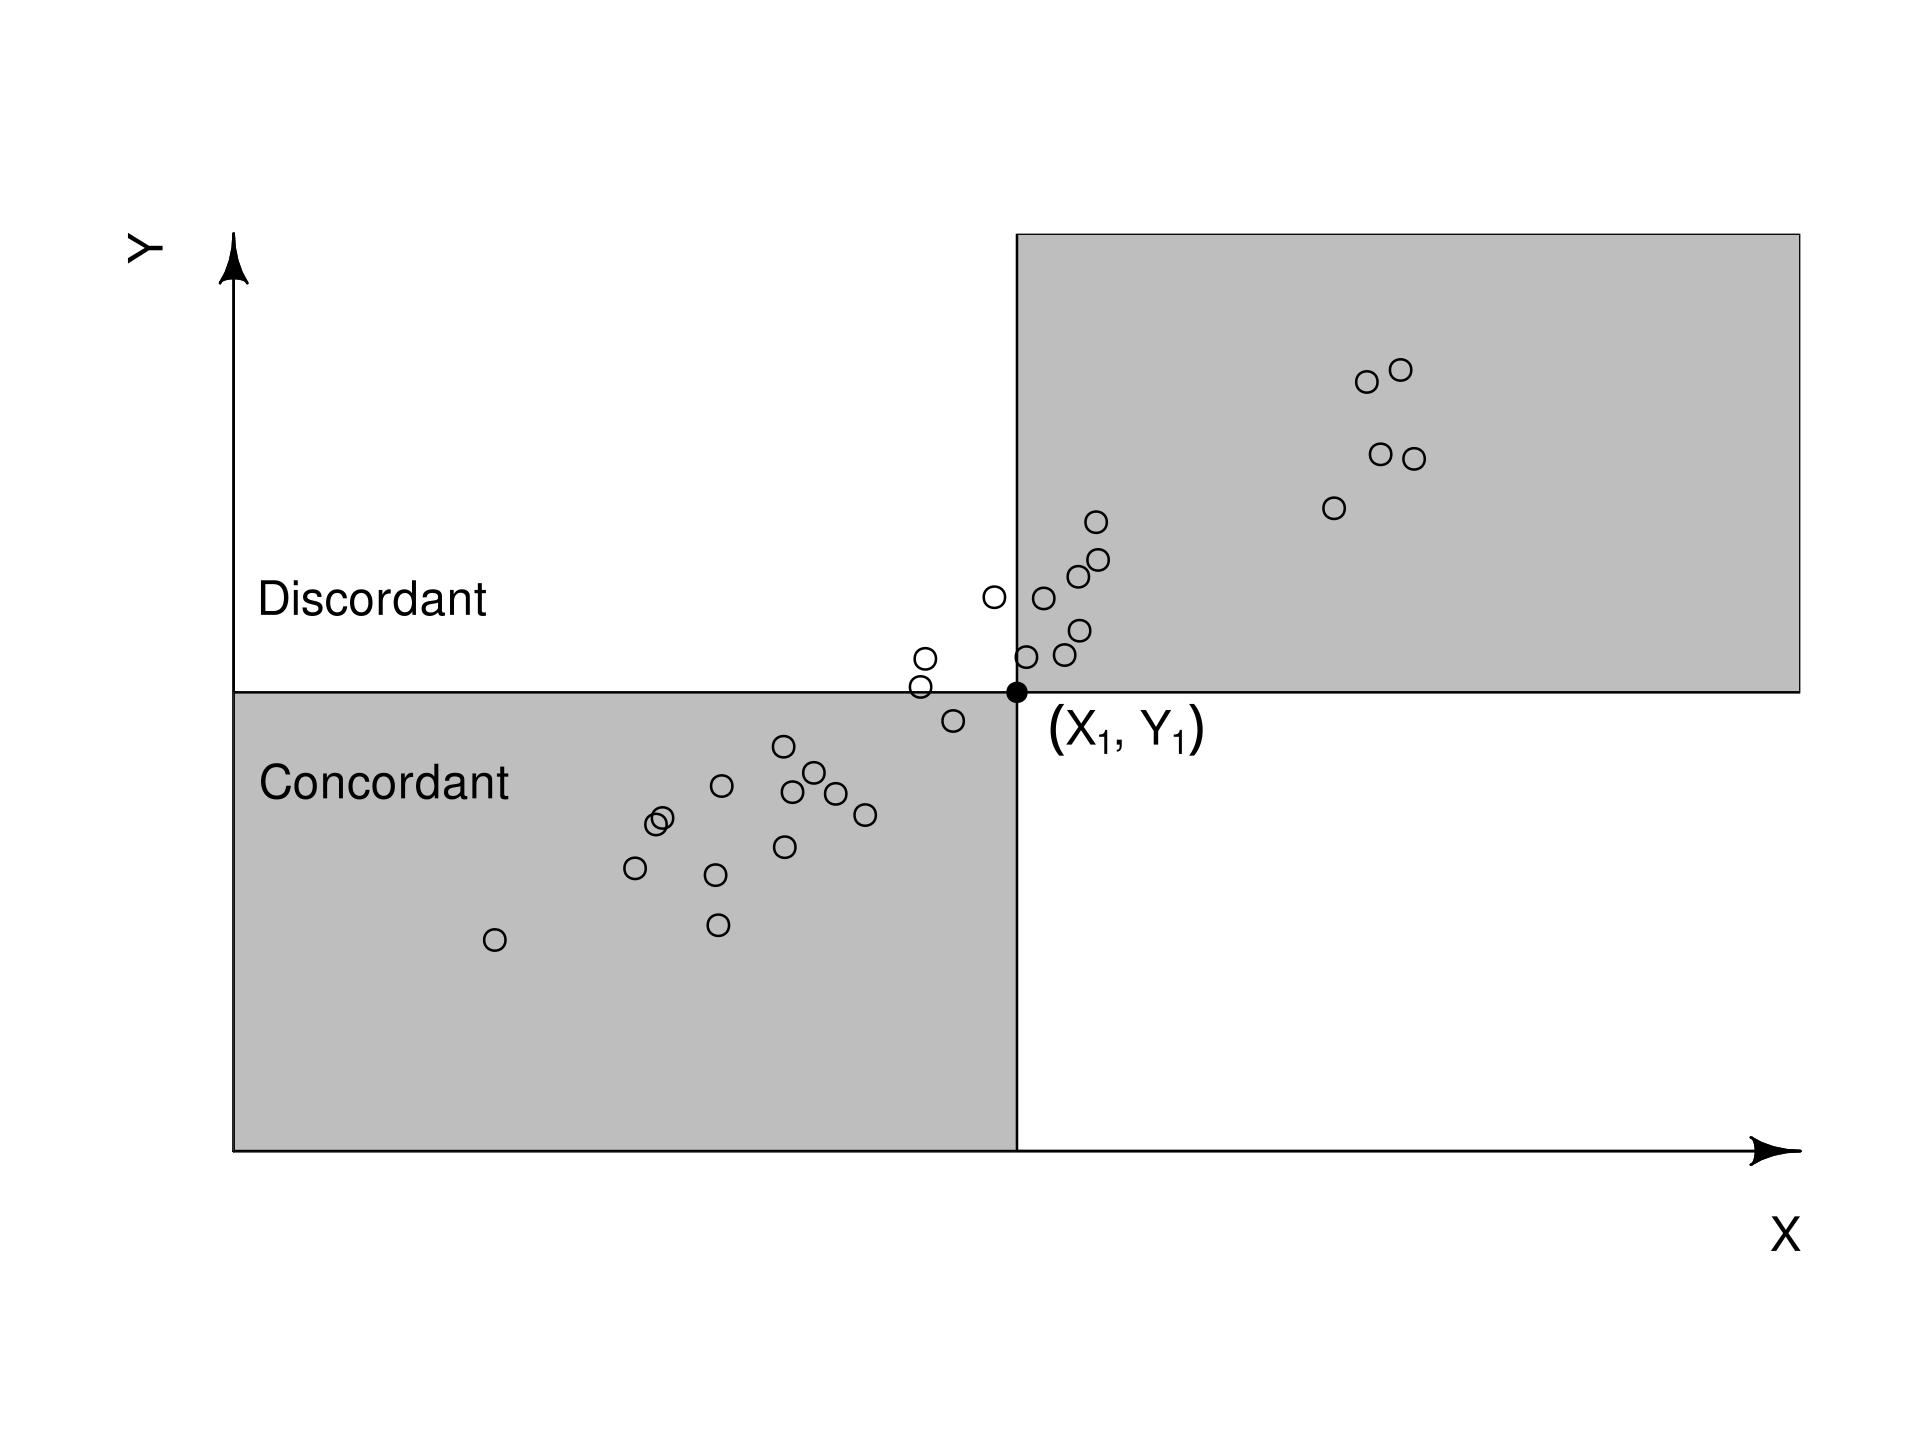
\includegraphics[width=0.5\textwidth]{figures/10-kendall-concordance.png}
  \caption{Kendall's $\tau$ 中一致与不一致的样本对。图片来自 \url{https://en.wikipedia.org/wiki/Kendall_rank_correlation_coefficient}}
  \label{fig:kendalls-tau}
\end{figure}

则 $\widehat\tau$ 本质上就是 $\tfrac{\text{一致样本对数}-\text{不一致样本对数}}{\text{总样本对数}}$ 。

\end{example}

\subsection{Mann--Whitney 统计量}

\begin{example}[Mann--Whitney 统计量]
这是一个两样本 U-统计量的例子。设 $X_1,\ldots,X_{n_1}\sim P$ i.i.d.、$Y_1,\ldots,Y_{n_2}\sim Q$ i.i.d.，且这些样本全体独立。``\textbf{\emph{Mann--Whitney 参数}}''考察 
$$\theta=P(X>Y)+\frac12 P(X=Y)$$
这个值经常用于假设检验，例如当 $X$ 来自``新药组''的某指标， $Y$ 来自``安慰剂组''，那么对假设 $\theta=0.5$ 进行检验能够判断两组是否存在系统性的区分。

取核函数 \[ h(x;y)=\mathbb I(x>y)+\frac12\mathbb I(x=y) \]两样本 U-统计量如下
\[\begin{aligned} U_{n_1,n_2}&=\frac1{n_1n_2}\sum_{j_1=1}^{n_1}\sum_{j_2=1}^{n_2}h(X_{j_1};Y_{j_2})\\ &=\frac1{n_1n_2}\sum_{j_1=1}^{n_1}\sum_{j_2=1}^{n_2}\Big(\mathbb I(X_{j_1}>Y_{j_2})+\frac12\mathbb I(X_{j_1}=Y_{j_2})\Big) \end{aligned}\]
将 $n_1n_2U_{n_1,n_2}$ 称作\textbf{\emph{Mann‑Whitney 统计量}} 。

\end{example}
\begin{remark}

\begin{itemize}
\tightlist
\item
  在机器学习领域的二分类问题中，如果记 $X_1,\dots,X_{n_1}$ 是分类器对正样本的打分、 $Y_1,\dots,Y_{n_2}$ 是对负样本打分，那么，基于这些样本绘制的 ROC 曲线，其\textbf{\emph{曲线下面积}} (AUC) 正是 $U_{n_1,n_2}$ 。例如，可参考早期文献 \cite{bamber1975}，或者机器学习相关资料，如 \cite{zhouzhihua2016} 的 §2.3.3 等。
\end{itemize}

% \href{https://www.zhihu.com/question/39840928}{如何理解机器学习和统计中的AUC？}

\begin{itemize}
\tightlist
\item
  如果将合样本 $X_1,\dots,X_{n_1},Y_1,\dots,Y_{n_2}$ 进行统一排序，并将每一样本在排序后的位次称作它的\textbf{\emph{秩 }}(rank)------当存在多个样本取相同的值，即所谓的 \textbf{\emph{结}} (ties)，我们用这些相同值样本的位次之平均作为它们的秩。即， $X_i$ 的秩为，
\end{itemize}
\[\begin{aligned} R_i &=\text{ 合样本中取值小于 $X_i$ 的个数} + \frac{\text{合样本中取值等于 $X_i$ 的个数} +1}2  \\&= \sum_{j_1=1}^{n_1} \mathbb{I}(X_{j_1} < X_i) \;+\; \sum_{j_2=1}^{n_2} \mathbb{I}(Y_{j_2} < X_i) \;+\; \frac{1}{2}\left( \sum_{j_1=1}^{n_1} \mathbb{I}(X_{j_1} = X_i) \;+\; \sum_{j_2=1}^{n_2} \mathbb{I}(Y_{j_2} = X_i) \;+\; 1 \right) \end{aligned}\]
那么，\textbf{\emph{Wilcoxon 秩和统计量}}定义为对所有 $X_i$ 的秩求和， $W_{n_1,n_2}=\sum_{i=1}^{n_1}R_i$。通过简单计算，我们得到\[\begin{aligned} W_{n_1,n_2} &= \sum_{j_1=1}^{n_1} \left( \sum_{k=1}^{n_1}\mathbb I(X_k<X_{j_1})+\sum_{l=1}^{n_2}\mathbb I(Y_l<X_{j_1})+\frac12\Biggl(\sum_{k=1}^{n_1}\mathbb I(X_k=X_{j_1})+\sum_{l=1}^{n_2}\mathbb I(Y_l=X_{j_1})+1\Biggr) \right) \\ &= \left(\sum_{j_1=1}^{n_1}\sum_{k=1}^{n_1}\mathbb I(X_k<X_{j_1})+\frac12\sum_{j_1=1}^{n_1}\sum_{k=1}^{n_1}\mathbb I(X_k=X_{j_1})\right) \\ &\qquad + \left(\sum_{j_1=1}^{n_1}\sum_{l=1}^{n_2}\mathbb I(Y_l<X_{j_1})+\frac12\sum_{j_1=1}^{n_1}\sum_{l=1}^{n_2}\mathbb I(Y_l=X_{j_1})\right) + \frac{n_1}{2} \\ &= \frac{n_1^2}{2} + \underbrace{\sum_{j_1=1}^{n_1}\sum_{l=1}^{n_2}\Bigl(\mathbb I(X_{j_1}>Y_l)+\frac12\mathbb I(X_{j_1}=Y_l)\Bigr)}_{=n_1n_2U_{n_1,n_2}} \;+\; \frac{n_1}{2} \\ &= n_1n_2U_{n_1,n_2} + \frac{n_1(n_1+1)}{2}. \end{aligned}\]这种统计量与 Mann‑Whitney 统计量仅相差一个 $\tfrac{n_1(n_1+1)}2$ ，因而二者在统计应用中可以视作是完全等价的。
\end{remark}


\subsection{最大均值差异 (MMD)}

本节是一个``齐一性检验''的例子，其目标是解决如下问题：给定取值于同一样本空间 $(\mathscr X,\mathscr B_x)$ 的两组独立样本 $X_1,\dots,X_{n_1}\sim P$ 、 $Y_1,\dots,Y_{n_2}\sim Q$ ，如何通过样本判断分布 $P$ 和 $Q$ 是否相同？

传统的方法，诸如 χ² 齐一性检验，对数据的限制太强，必须要求数据是有限离散的分离数据，对连续情况必须要分组处理；而且，这一方法也很难应用在高维的、结构复杂的数据上。\textbf{\emph{最大均值差异}} (Maximum Mean Discrepancy, MMD) 是一种基于核的距离度量，它通过将分布映射到\href{https://en.wikipedia.org/wiki/Reproducing_kernel_Hilbert_space}{再生核 Hilbert 空间}（RKHS）来比较它们之间的差异；原则上，只需要找到一个核 $k$ ，那么无论数据是连续或是高维，都可以定义出 MMD。

\begin{example}[最大均值差异（MMD）]\label{ex:ch10:mmd}
设 $\mathscr X$ 上有对称正定的核函数
\[k:\mathscr X\times \mathscr X\to\mathbb R\]
由 \href{https://en.wikipedia.org/wiki/Reproducing_kernel_Hilbert_space\#Moore\%E2\%80\%93Aronszajn_theorem}{Moore--Aronszajn 定理}，在 $\mathscr X$ 上存在唯一的 RKHS 空间 $\mathscr H_k$ 以 $k$ 为再生核。对每个分布 $P$ ，它在 $\mathscr H_k$ 中有均值嵌入 (mean embedding)：
\[
\mu_P=\mathbb E_{X\sim P}[k(\cdot,X)]=\int_{\mathscr X}k(\cdot,x)\mathrm{d}P(x).
\]

MMD 定义为两个嵌入之间的 Hilbert 空间距离：
\[
\mathrm{MMD}_k^2(P,Q)=\|\mu_P-\mu_Q\|^2_{\mathscr H_k}.
\]
在实践中，我们往往把范数平方展开，从而得到下面的形式：记独立样本 $X,X'\sim P$ 、 $Y,Y'\sim Q$ ，那么
\[
\mathrm{MMD}_k^2(P,Q) = \mathbb{E}_{X,X'\sim P}[k(X,X')] + \mathbb{E}_{Y,Y'\sim Q}[k(Y,Y')] - 2\mathbb{E}_{X\sim P, Y\sim Q}[k(X,Y)].
\]
为了配合上述形式，我们设两组样本是配对的：$(X_i, Y_i),~i=1,\ldots,n$，考虑 U-统计量核
\[
h_k^{(\mathrm{MMD})}\bigl((x_1,y_1), (x_2,y_2)\bigr) = k(x_1,x_2) + k(y_1,y_2) - k(x_1,y_2) - k(x_2,y_1).
\]
则 U-统计量如下：
\[\begin{aligned}\widehat{\mathrm{MMD}}_{k}^2 &= \binom{n}{2}^{-1} \sum_{1\le i<j\le n} h_k^{(\mathrm{MMD})}\bigl((X_i,Y_i), (X_j,Y_j)\bigr)\\ &= \frac{2}{n(n-1)} \sum_{1\le i<j\le n} k(X_i,X_j) \;+\; \frac{2}{n(n-1)} \sum_{1\le i<j\le n} k(Y_i,Y_j) \;-\; \frac{2}{n(n-1)} \sum_{1\le i<j\le n} \bigl(k(X_i,Y_j)+k(X_j,Y_i)\bigr)\\ &= \frac{2}{n(n-1)} \sum_{1\le i<j\le n} k(X_i,X_j) + \frac{2}{n(n-1)} \sum_{1\le i<j\le n} k(Y_i,Y_j) - \frac2{n(n-1)} \sum_{i\neq j} k(X_i,Y_j) \end{aligned}\]

我们后文中会回顾这个例子，该例的特点在于：在 $P=Q$ 的原假设下， $\mathrm{MMD}_k^2(P,Q)=0$ ，此时 $\widehat{\mathrm{MMD}}_{k}^2$ 是一阶退化的 U-统计量。

% 参考阅读：

% \href{https://www.zhihu.com/question/386309435/answer/1973074816077682003}{如何衡量两个「任意数据集」间的相似度？}

% \href{https://zhuanlan.zhihu.com/p/679276071}{迁移学习简介之最大均值差异（Maximum Mean Discrepancy）}

\end{example}

\subsection{Hilbert--Schmidt 独立性准则 (HSIC)}

上一节是一个齐一性检验的例子，本节我们来看看独立性检验。\textbf{\emph{Hilbert‑Schmidt 独立性准则}} 的基本思想和 MMD 类似，都是将分布放在 RKHS 空间中进行研究。

\begin{example}[Hilbert--Schmidt 独立性准则（HSIC）]\label{ex:ch10:hsic}
设 $X$ 取值于 $\mathscr X$、$Y$ 取值于 $\mathscr Y$，给定对称、正定的核函数
\[
k:\mathscr X\times \mathscr X\to \mathbb R,\quad l:\mathscr Y\times \mathscr Y\to \mathbb R.
\]
二者分别对应的 RKHS 记作 $\mathscr H_k$ 和 $\mathscr H_l$ 。定义联合分布 $P_{XY}$ 的均值嵌入为
\[\begin{aligned} \mu_{P_{XY}}&=\mathbb{E}_{X,Y}[k(\cdot,X)\otimes l(\cdot,Y)]\\ &=\int_{\mathscr X\times\mathscr Y}k(\cdot ,x)l(\cdot,y)\mathrm dP_{XY}(x,y) \end{aligned}\]
这里 $k(\cdot,X)\otimes l(\cdot,Y)$ 应该理解成一个二元函数：
\[
(x,y)\mapsto (k(\cdot,X)\otimes l(\cdot,Y))(x,y)=k(x,X)l(y,Y).
\]
而 $\mu_{P_{XY}}$ 实际上是 $\mathscr H_k\otimes \mathscr H_l$ 中的元素。

HSIC 定义为 \cite{gretton2005,gretton2008}：
\[
\mathrm{HSIC}_{k,l} = \|\mu_{P_{XY}} - \mu_{P_X} \otimes \mu_{P_Y}\|_{\mathscr{H}_k\otimes\mathscr{H}_l}^2.
\]

可见它其实就是 $P_{XY}$ 与 $P_X\otimes P_Y$ 在张量积空间 $\mathscr H_k\otimes \mathscr H_l$ 上的 MMD。展开范数平方，有下述更加简单的形式，
\[\begin{aligned} \mathrm{HSIC}_{k,l} &= \mathbb{E}_{X,X',Y,Y'}\bigl[k(X,X')l(Y,Y')\bigr] + \mathbb{E}_{X,X'}[k(X,X')]\mathbb{E}_{Y,Y'}[l(Y,Y')] - 2\mathbb{E}_{X,Y}\bigl[\mathbb{E}_{X'}[k(X,X')]\mathbb{E}_{Y'}[l(Y,Y')]\bigr]\\  \end{aligned}\]

对 $z_a = (x_a, y_a),\ a=1,2,3,4$ ，我们构造下面的四阶 U-统计量核 ：
\[\begin{aligned}h_{k,l}^{(\mathrm{HSIC})}(z_1, z_2, z_3, z_4) & = \frac{1}{4} h_k^{(\mathrm{MMD})}((x_1,x_3),(x_2,x_4)) h_l^{(\mathrm{MMD})}((y_1,y_3),(y_2,y_4))\\ &=\frac{1}{4} \Big(K_{12} + K_{34} - K_{14} - K_{23}\Big)\Big(L_{12} + L_{34} - L_{14} - L_{23}\Big)  \end{aligned}\]
其中 $K_{ij}=k(X_i,X_j)$ 代表 Gram 矩阵的 $i,j$ 元； $L_{ij}$ 同理；注意这个核非对称，那么 U-统计量应该写作
\[
\widehat{\mathrm{HSIC}}_{k,l}= \binom{n}{4}^{-1} \frac1{4!}\sum_{\substack{1\le j_1 , j_2 , j_3 , j_4 \le n\\ j_1,j_2,j_3,j_4\text{ 互不相同 }}} h_{k,l}^{(\text{HSIC})}(Z_{j_1}, Z_{j_2}, Z_{j_3}, Z_{j_4}).
\]
也可以用下面这个等价的对称核：
\[
h_{k,l}(Z_1,Z_2,Z_3,Z_4) = \frac{1}{4!}\sum_{\pi \in S_4} \Bigl(K_{\pi(1)\pi(2)} L_{\pi(1)\pi(2)} + K_{\pi(1)\pi(2)} L_{\pi(3)\pi(4)} - 2K_{\pi(1)\pi(2)} L_{\pi(1)\pi(3)}\Bigr).
\]

经过极其繁琐的展开， $\widehat{\mathrm{HSIC}}_{k,l}$ 最终能化简成\[\begin{aligned} \widehat{\mathrm{HSIC}}_{k,l} &= \frac{1}{n(n-1)} \sum_{1 \le j_1 \neq j_2 \le n} k(x_{j_1}, x_{j_2})\, l(y_{j_1}, y_{j_2}) \\ &\quad - \frac{2}{n(n-1)(n-2)} \sum_{\substack{1 \le j_1,j_2,j_3 \le n \\ j_1,j_2,j_3\ \text{互不相等}}} k(x_{j_1}, x_{j_2})\, l(y_{j_1}, y_{j_3}) \\ &\quad + \frac{1}{n(n-1)(n-2)(n-3)} \sum_{\substack{1 \le j_1,j_2,j_3,j_4 \le n \\ j_1,j_2,j_3,j_4\ \text{互不相等}}} k(x_{j_1}, x_{j_2})l(y_{j_3}, y_{j_4}). \end{aligned}\]
这个估计量可以参考 \cite{song2007,song2012}。


与例~\ref{ex:ch10:mmd} 相同，当 $X$ 和 $Y$ 独立时， $\mathrm{HSIC}_{k,l}=0$ ，可以证明 $\widehat{\mathrm{HSIC}}_{k,l}$ 也是一个退化的 U-统计量。

% 相关阅读：\href{https://spaces.ac.cn/archives/6910}{HSIC简介：一个有意思的判断相关性的思路 - 科学空间\textbar Scientific Spaces}。

\end{example}

\section{U-统计量的方差}

设 $X_1,\dots,X_m\sim P$ i.i.d.， U-统计量 $U_n$ 的核函数对称，并满足 $\mathbb E_P[h^2(X_1,\dots,X_m)]<\infty$ ，那么，令 $h_0=\theta=\mathbb E_P[h(X_1,\dots,X_m)]$

并对 $k=1,2,\dots,m$ ， 令
\[\begin{aligned} h_k(x_1,\dots,x_k)&=\mathbb E_P[h(x_1,\dots,x_k,X_{k+1},\dots,X_m)]\\ &=\mathbb E_P\Big[h(X_1,\dots,X_m)\ \Big|\  X_1=x_1,\dots,X_k=x_k\Big]\\ \end{aligned}\]
即固定前 $k$ 个变量，对剩余变量取平均。

将每个 $h_k$ 中心化，记
\[
\widetilde h_k(x_1,\dots,x_k)=h_{k}(x_1,\dots,x_k)-\theta.
\]
那么 $\mathbb E_P[h_k(X_1,\dots,X_k)]=0$ 。

再记
\[
\xi_k := \mathrm{Var}[h_k(X_1,\ldots,X_k)] = \mathbb{E}_P\Bigl[\widetilde{h}_k^2(X_1,\dots,X_k)\Bigr].
\]
在 $\mathbb E_P[h^2(X_1,\dots,X_m)]<\infty$ 的条件下，各 $\xi_k$ 是存在且有限的；实际上，易知方差随着固定变量数增加而单调不减
\[0 = \xi_0 \le \xi_1 \le \xi_2 \le \cdots \le \xi_m\]
这些 $\xi_k$ 衡量了 ``在已知 $k$ 个样本时，条件期望的变异程度''：
\begin{itemize}
\tightlist
\item
  若 $\xi_k$ 很大，说明 $k$ 个变量的观测会显著改变核 $h$ 的值，从而对 U-统计量产生较大的影响；
\item
  若 $\xi_k$ 很小，说明固定 $k$ 个变量后， $h$ 取值仍然接近于 $\theta$ ，不会发生较大的转变。
\end{itemize}

还有一点是，设 $\{1,\dots,n\}$ 的两组 $m$ 元指标子集 $I=\{\alpha_1,\dots,\alpha_m\}$ 和 $J=\{\beta_1,\dots,\beta_m\}$ 仅有 $k$ 个公共元素，那么
\[\begin{aligned} \mathrm{Cov}\big[ h(X_I),h(X_J)\big]&=\mathbb E\Big[\widetilde h(X_I)\widetilde h(X_J)\Big]\\ &=\mathbb E\Big[\mathbb E\Big[\widetilde h(X_I)\Big|X_{I\cap J}\Big]\mathbb E\Big[\widetilde h(X_J)\Big|I\cap J\Big]\Big]\\ &=\mathbb E\Big[\widetilde h^2_k(X_1,\dots,X_k)\Big]\\ &=\xi_k \end{aligned}\]
即：协方差仅依赖于指标集的公共元素个数。这是很关键的一步：当固定 $I$ 时，所有 $m$ 元指标子集 $J$ 中，与 $I$ 恰有 $k$ 个公共元的 $J$ 共有 $\binom mk\binom {n-m}{m-k}$个。通过以上这些准备，立即推出
\[\begin{aligned} \mathrm{Var}(U_n)&=\mathbb E_P\Big[(U_n-\mathbb E_P[U_n])^2\Big]\\ &= \binom{n}{m}^{-2} \sum_{I} \sum_{J} \mathrm {Cov}\bigl[h(X_I),h(X_J)\bigr]\\ &=\binom{n}{m}^{-2} \sum_I\sum_{k=1}^{m}\binom mk\binom{n-m}{m-k}\xi_k\\ &=\binom{n}{m}^{-1} \sum_{k=1}^{m}\binom mk\binom{n-m}{m-k}\xi_k \end{aligned}\]

我们写作定理。

\begin{theorem}[U-统计量的方差公式]
\label{thm:ch10:u-statistic-variance}

设 U -统计量的核 $h$ 对称，且 $\mathbb E[h^2(X_1,\dots,X_m)]<\infty$ ，那么由式~\eqref{eq:ch10a:tag-2} 定义的 U-统计量的方差为
\[\begin{aligned} \mathrm{Var}(U_n)=\binom{n}{m}^{-1} \sum_{k=1}^{m}\binom mk\binom{n-m}{m-k}\xi_k \end{aligned}\]
\end{theorem}

\begin{example}[样本方差的方差]
假定总体四阶矩有限，以 $\mu=\mathbb E_P[X]$ 记总体均值、 $\mu_k:=\mathbb E_P[(X-\mathbb E_P[X])^k]$ 记总体 $k$ 阶中心距，那么对 $h(x_1,x_2)=\tfrac{(x_1-x_2)^2}{2}$ ，有
\[\begin{aligned} h_1(x_1)&=\mathbb E_P[h(x_1,X_2)]=\frac12\mathbb E_P[(x_1-X_2)^2]\\ &=\frac12\mathbb E_P[(x_1-\mu)^2+(\mu-X_2)^2]\\ &=\frac12((x_1-\mu)^2+\mu_2) \end{aligned}\]
从而 \[ \xi_1=\mathrm{Var}[h_1(X_1)] = \frac14 \mathrm{Var}\!\big[(X_1-\mu)^2\big]=\frac{\mu_4-\mu_2^2}4 \]而
\[\begin{aligned} \xi_2&=\mathrm{Var}_P[h(X_1,X_2)] \\&= \mathbb{E}[h(X_1,X_2)^2] - (\mathbb{E}[h(X_1,X_2)])^2 \\ &= \frac14 \mathbb{E}[(X_1-X_2)^4] - \left( \frac12 \mathbb{E}[(X_1-X_2)^2] \right)^2 \\ &= \frac14 \mathbb{E}[((X_1-\mu)-(X_2-\mu))^4] - \mu_2^2 \\ &= \frac14 ( \mu_4 + 6\mu_2^2 + \mu_4 ) - \mu_2^2 \\ &= \frac{\mu_4 + \mu_2^2}{2} \end{aligned}\]
那么根据定理~\ref{thm:ch10:u-statistic-variance}，样本方差的方差为
\[\begin{aligned}\mathrm{Var}_P\left[\frac1{n-1}\sum_{j=1}^n(X_j-\bar X)^2\right]&=\binom{n}{2}^{-1} \sum_{k=1}^{2} \binom{2}{k} \binom{n-2}{2-k} \xi_k \\ &= \frac{4(n-2)}{n(n-1)}\xi_1 + \frac{2}{n(n-1)}\xi_2\\ &=\frac{\mu_4}{n} - \frac{n-3}{n(n-1)}\mu_2^2 \end{aligned}\]

\end{example}

\section{U-统计量的相合性}

利用方差公式容易得出如下推论

\begin{corollary}\label{cor:ch10:u-statistic-variance-order}
若 $\xi_1=\cdots=\xi_{r-1}=0$，$\xi_r>0$，那么
\[\mathrm{Var}[U_n]=\frac{r!}{n^r}{\binom mr}^2\xi_r+O\left(\frac1{n^{r+1}}\right)\]\end{corollary}

\begin{proof}

只需注意到对任意 $k=1,\dots,m$ ，定理~\ref{thm:ch10:u-statistic-variance} 中 $\xi_k$ 的系数
\[\begin{aligned} \binom{n}{m}^{-1} \binom mk\binom{n-m}{m-k}&=\frac{(n-m)!{\color{DarkRed}{m!}}}{n!}\frac{\color{DarkRed}{m!}}{\color{DarkRed}{k!(m-k)!}}\frac{(n-m)!}{{\color{DarkRed}{(m-k)!}}(n-2m+k)!}\\ &
  ={\color{DarkRed}{k!{\binom mk}^2}}\frac{(n-m)(n-m-1)\cdots(n-2m+k+1)}{n(n-1)\cdots (n-m+1)}\\ &=k!{\binom mk}^2\left(\frac1{n^k}+O\left(\frac1{n^{k+1}}\right)\right)\\ &=\frac{k!}{n^k}{\binom mk}^2+O\left(\frac1{n^{k+1}}\right) \end{aligned}\]
\end{proof}

这个推论告诉我们：

\begin{itemize}
\tightlist
\item
  若 $\xi_1>0$ ，那么方差至少以 $O(1/n)$ 的速率衰减，从而 $U_n-\theta=O_P(n^{-1/2})$ ；若 $\xi_1=0$ ，我们称 $U_n$ (一阶) 退化。
\item
  若 $\xi_1=0$ 但 $\xi_2>0$ ，那么方差至少以 $O(1/n^2)$ 的速率衰减，从而 $U_n-\theta=O_P(n^{-1})$ ；
\item
  依此类推，如果前 $r-1$ 项都为 0： $\xi_1=\cdots=\xi_{r-1}=0$ ，则方差至少以 $O(1/n^r)$ 衰减，从而 $U_n-\theta=O_P(n^{-r/2})$ 。
\end{itemize}
这论证了 $U_n\overset{P}\to \theta$ ，即 $U_n$ 是 (弱) 相合估计。

最后要补充的是： $U_n$ 不仅依概率收敛于 $\theta$ ，a.s. 收敛（强相合）也是成立的：

\begin{theorem}[U-统计量的强相合性]\label{thm:ch10:u-statistic-strong-consistency}

设 $\mathbb E_P[|h(X_1,\dots,X_n)|]<\infty$ ，那么 $U_n\overset{\text{a.s.}}\to\theta$ 。

\end{theorem}

\begin{remark}
U-统计量强相合性的原始结果可参见 \cite{berk1966} 与 \cite{arvesen1969}。定理~\ref{thm:ch10:u-statistic-strong-consistency} 有多种证明方法，例如 \cite{lee1990} 一书的 §3.4 就给出了三种不同的证明。限于篇幅，我们这里介绍其中最为简洁优雅的第三种证明。亦可参考~\cite{chenxiru2012} 的 §2.4.1 。
\end{remark}

\begin{proof}

对任意 $\epsilon > 0$ ，定义
\[\begin{aligned} U(\epsilon) &:= \bigl\{ U_n > \theta + \epsilon \text{ 发生无穷多次} \bigr\}\\ L(\epsilon) &:= \bigl\{ U_n < \theta - \epsilon \text{ 发生无穷多次} \bigr\} \end{aligned}\]
用集合论的语言，
\[\begin{aligned} U(\epsilon) &= \bigcap_{n=1}^{\infty} \bigcup_{m=n}^{\infty} \{ U_m > \theta + \epsilon \}\\ L(\epsilon) &= \bigcap_{n=1}^{\infty} \bigcup_{m=n}^{\infty} \{ U_m < \theta + \epsilon \}\\  \end{aligned}\]
由于 U-统计量 $U_n$ 的性质，上面两个事件都是可排列的 (permutable)，即，只对有限多个 $X_j$ 交换次序，那么对足够大的 $m$ ，U-统计量 $U_m$ 是不发生改变的，从而不影响``发生无穷多次''。由 \href{https://en.wikipedia.org/wiki/Hewitt\%E2\%80\%93Savage_zero\%E2\%80\%93one_law}{Hewitt‑Savage 0‑1 律}， $U(\epsilon)$ 和 $L(\epsilon)$ 的概率要么是 0 要么是 1；这里的``概率''视作是 $X$ 所在概率空间的无穷乘积空间上的概率测度。

设 $T_n:=\{X_{(1)},\dots,X_{(n)}\}$ 是次序统计量，考虑 $\sigma$-代数族
\[
\mathscr F_n:=\sigma(T_n,X_{n+1},X_{n+2},\dots).
\]

那么 $\mathscr F_n\supset \mathscr F_{n+1}$，于是\[ U_{n+1}=\mathbb E_P[h(X_1,\dots,X_m)\mid T_{n+1}]=\mathbb E_P[h(X_1,\dots,X_m)\mid \mathscr F_{n+1}]=\mathbb E_P[U_n\mid \mathscr F_n]\quad \text{a.s.} \]

可知 $U_n$ 构成反向鞅 (Reverse Martingale)，由鞅收敛定理，存在随机变量 $U_\infty$ 使得
\[
U_n \xrightarrow{\text{a.s. 且 } L_1} U_\infty \quad \text{ 当 } n \to \infty.
\]

由于 $\mathbb{E}[U_n] = \theta$ ，不可能以概率 1 发生 $U_n > \theta + \epsilon$ 无穷多次，如若不然，
\[ \theta = \lim_{n\to\infty} \mathbb{E}[U_n]=\mathbb E[U_\infty]\ge \theta + \epsilon \]矛盾。所以 $U(\epsilon)$ 发生的概率是 0，同理， $L(\epsilon)$ 亦如此。而`` $U_n$ 不收敛于 $\theta$ ''的样本点可以表示为 $\bigcup_{k=1}^{\infty} \bigl( U(1/k) \cup L(1/k) \bigr)$ ，这发生的概率仍然是 0。

\end{proof}
